\chapter{Sezione sperimentale}
\label{sec:5_esperimenti}

In questo capitolo viene presentata l'analisi sperimentale svolta per valutare l'approccio multi-agente proposto nella tesi. La prima sezione espone le scelte sperimentali adottate nell'implementazione degli ambienti e dell'algoritmo, oltre alla configurazione degli addestramenti e la presentazione delle metriche di valutazione. La seconda sezione invece presenta e analizza i risultati ottenuti.

\section{Tecnologie implementative}

Nell'implementazione ed esecuzione degli esperimenti sono state effettuate scelte tecnologiche per realizzare lo studio. La scelta più importante è stata l'uso di Python come linguaggio di programmazione, per via della sua popolarità nell'ambito del machine learning e nello specifico nell'apprendimento per rinforzo. È stata poi scelta la libreria RLlib, presentata in \cite{Liang2018}, come base da cui implementare gli ambienti ed eseguire gli esperimenti. RLlib\footnote{\url{https://docs.ray.io/en/latest/rllib/index.html}} è una libreria open source per l'apprendimento per rinforzo che implementa algoritmi ottimizzati per utilizzare accelerazione hardware, tramite il framework PyTorch introdotto da \cite{Ansel2024}. Rispetto ad altre librerie è stata preferita perché incorpora funzionalità che si adattano
allo scenario di FaaS decentralizzato: gli algoritmi sono implementati anche in versione decentralizzata, con la possibilità di sviluppare ambienti multi-agente. RLlib è basato su Ray \cite{Moritz2018}, un framework open source che supporta l'esecuzione decentralizzata e distribuita di applicazioni scritte in Python e dedicate al machine learning. È stata utilizzata nello specifico la versione 2.10.0 di RLlib. La \Cref{fig:5_ray_rllib_architecture} mostra l'architettura della libreria.

\begin{figure}[ht]
    \centering
    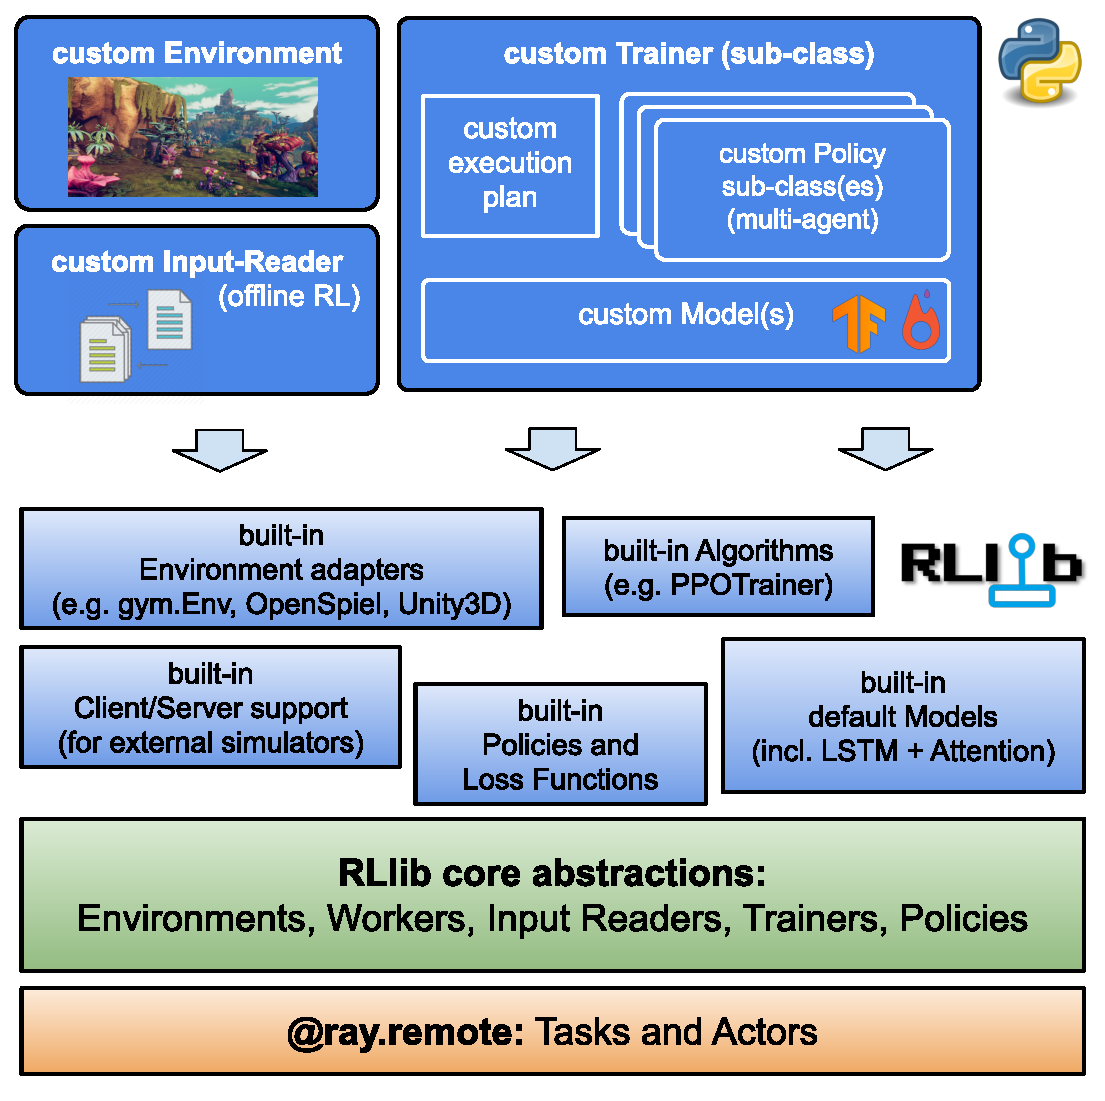
\includegraphics[width=.6\linewidth]{assets/5/ray_rllib_architecture.pdf}
    \caption[Architettura della libreria RLlib]{Architettura della libreria RLlib. Fonte: \url{https://docs.ray.io/en/latest/rllib/index.html}}
    \label{fig:5_ray_rllib_architecture}
\end{figure}

Gli ambienti sono stati implementati seguendo le API multi-agente definite da RLlib, a loro volta basate su Gymnasium, l'API standard de-facto per gli ambienti per l'apprendimento per rinforzo in Python, approfondita in \cite{Towers2024}.

Nell'implementazione sono state inoltre utilizzate le seguenti librerie: NumPy per la gestione degli array, presentata in \cite{Harris2020}, Pandas per la gestione dei dati nello scenario reale, presentata in \cite{Mckinney2010} e \cite{Pandas2024}, e Matplotlib per la produzione dei grafici presenti nel documento, introdotto in \cite{Hunter2007}.

\section{Configurazione e valutazione degli esperimenti}

L'obiettivo dell'analisi sperimentale è di validare la realizzabilità di un ambiente multi-agente per la distribuzione del carico con l'algoritmo PPO, nelle due modalità multi-agente descritte in \Cref{sec:2_rl_ppo_choices}. Nello specifico, l'analisi vuole dimostrare che, al crescere della complessità degli ambienti modellati nel \Cref{sec:4_modellazione}, ossia permettendo di inoltrare le richieste, gli agenti siano in grado di processare un maggior numero di richieste, a fronte di carichi in ingresso di natura diversa, le cui tipologie sono dettagliate nella sottosezione seguente. La configurazione degli esperimenti è stata attentamente progettata per assicurare risultati che siano coerenti e soprattutto riproducibili.

\subsection{Configurazione degli ambienti}

I tre ambienti modellati sono stati configurati nel seguente modo:

\begin{itemize}
    \item Ogni agente ha la stessa capacità di coda locale per ogni passo fissa a 100, per cui $q^\textnormal{MAX} \coloneqq 100$.

    \item Il carico $R^\textnormal{IN}$ in ingresso ad ogni agente $n \in \mathcal{N}$ al $t$-esimo passo può assumere valori nell'intervallo $[0, 150]$.

    \item Ogni ambiente ha due agenti $|\mathcal{N}| = 2$. Nel caso dell'ambiente asimmetrico, un agente può inoltrare, mentre l'altro può solo ricevere le richieste inoltrate.
\end{itemize}

La scelte di $q^\textnormal{MAX}$ e dell'intervallo di $R^\textnormal{IN}$ sono state effettuate sulla base di osservazioni empiriche per garantire dei carichi gestibili per i due agenti. Come anticipato nella \Cref{sec:4_dinamica_ambienti}, l'ambiente è di tipo episodico da 288 passi.

\subsection{Scenari}
\label{sec:5_scenari}

Nell'esecuzione degli esperimenti, per una successiva valutazione di PPO ad apprendere politiche ottimali di distribuzione, un passo importante è stata la scelta delle richieste da fornire in ingresso a ogni agente dell'ambiente, sia in fase di addestramento sia in fase di valutazione. Per tale scopo sono stati definiti tre scenari, caratterizzati dalla modalità di generazione delle richieste in ingresso. Il criterio di definizione ha l'obiettivo di presentare agli agenti scenari che esprimano situazioni multiformi, fornendo in questo modo una visione più ampia dei comportamenti appresi dall'algoritmo nelle situazioni proposte. Inoltre, gli scenari sono stati progettati cercando di sottoporre gli agenti a contesti di lavoro di varie difficoltà e forme. Nello specifico, gli scenari definiti sono:

\begin{itemize}
    \item \textbf{Scenario reale}: gli agenti sono sottoposti a carichi provenienti da dati reali di traffico in ingresso, selezionati ed elaborati come descritto nelle sezioni successive.

    \item \textbf{Scenari sintetici}: gli agenti sono sottoposti a carichi generati artificialmente che non hanno una corrispondenza reale ma sono costruiti con delle caratteristiche simili ai carichi reali. Sono stati definiti due scenari per questa tipologia:

        \begin{itemize}
            \item \textbf{Scenario sintetico sinusoidale}: ogni agente è sottoposto a un carico generato seguendo una forma sinusoidale, con l'aggiunta di rumore.

            \item \textbf{Scenario sintetico gaussiano}: ogni agente è sottoposto da un carico generato seguendo una distribuzione normale.
        \end{itemize}
\end{itemize}

Per la durata di un intero episodio, per ogni agente sono generate (o estratte in caso di scenario reale) tracce con in media \numprint{17000}-\numprint{18000} richieste. I tre scenari hanno le seguenti caratteristiche in comune: una media di richieste di circa 60 per passo, deviazione standard di 30 (solo per lo scenario sintetico gaussiano e reale) e di 60 (scenario sintetico sinusoidale), mentre la deviazione standard della somma delle richieste è di \numprint{7500} (scenario reale) e \numprint{750} (scenari sintetici). Sono pertanto scenari diversi che pongono sfide di natura diversa agli agenti.

È importante sottolineare che in ogni fase di addestramento vengono estratte delle tracce da uno scenario selezionato all'avvio dell'esperimento. Questo significa che non è stato previsto che un agente venga addestrato con tracce di uno scenario diverso dall'altro agente. Lo stesso avviene per la valutazione, con la differenza che un agente può essere valutato più volte selezionando scenari alternativi a quello di addestramento.

\subsubsection{Scenario reale}
\label{sec:5_scenario_reale}

Lo scenario reale è definito dall'uso del sottoinsieme di richieste pubblicate e analizzate in \cite{Shahrad2020} e rilasciate su GitHub\footnote{\url{https://github.com/Azure/AzurePublicDataset}}. Le richieste, o ``tracce'' seguendo la terminologia del set di dati considerato, sono un sottoinsieme registrato dal 15 al 28 Luglio 2019 sull'intera infrastruttura di Microsoft Azure Functions. Il dataset cattura il carico in ingresso FaaS caratterizzato dalle proprietà intrinseche delle applicazioni e delle funzioni, e non dalle caratteristiche della piattaforma sottostante. Questo ha permesso di utilizzare le richieste raccolte così come sono nell'ambiente DFaaS simulato. I dati raccolti e pubblicati comprendono informazioni su quante volte al minuto viene invocata una funzione e per quale categoria di trigger\footnote{I trigger sono la causa di esecuzione di una funzione, definiscono come una funzione viene invocata. Azure Functions supporta decine di trigger, ma nel set di dati sono raggruppati in 7 classi.}, come le funzioni sono organizzate in applicazioni e a quali utenti sono associate, la distribuzione dei tempi di esecuzione per funzione e la distribuzione dell'utilizzo della memoria per applicazione. Per lo studio esplorativo di questa tesi, sono state considerate solo le invocazioni causate dal trigger HTTP, perché sono le più affini all'architettura e funzionamento di DFaaS. Due esempi di questa tipologia di tracce sono mostrate in \Cref{fig:5_real_traces}.

\begin{figure}
    \centering

    \begin{subfigure}{.95\textwidth}
        \centering
        \includegraphics[width=\linewidth]{assets/5/requests_9dc54e.pdf}
        \caption{Traccia della funzione 9dc54e.}
        \label{fig:5_real_traces_9dc54e}
    \end{subfigure}

    \begin{subfigure}{.95\textwidth}
        \centering
        \includegraphics[width=\linewidth]{assets/5/requests_f2d88b.pdf}
        \caption{Traccia della funzione f2d88b.}
        \label{fig:5_real_traces_f2d88b}
    \end{subfigure}
    
    \caption[Esempio di invocazioni di due funzioni dal set di dati reale]{Esempio di invocazioni di due funzioni registrate il 15 Luglio 2019 e scatenate dal trigger HTTP. Per ognuna sono indicati gli ultimi tre byte dell'hash di identificazione.}
    \label{fig:5_real_traces}
\end{figure}

Il set di dati è costituito da 14 file in formato CSV, ognuno dei quali caratterizza le invocazioni relative a funzioni per un giorno preciso. Per ogni traccia registrata è presente l'identificativo della funzione, dell'applicazione e dell'utente (il proprietario). All'interno della piattaforma Azure Functions, le funzioni sono logicamente raggruppate in applicazioni, e un'applicazione può comprendere una o più funzioni. Un unico utente può essere legato a più di una applicazione. È importante sottolineare che funzioni identiche possono appartenere a diverse applicazioni, e una stessa applicazione a più utenti (ognuno dei quali con una propria copia). Il set di dati è stato reso anonimo processando tutti gli identificativi con HMAC-SHA256 e un salt\footnote{Una sequenza casuale di bit aggiunti alla funzione di hash per evitare che due stessi input vengano mappati allo stesso hash.} segreto diverso per ogni colonna. Di conseguenza due applicazioni identiche ma con diversi proprietari sono identificati da hash diversi, e lo stesso vale per due funzioni identiche che appartengono ad applicazioni diverse. Tuttavia gli hash sono coerenti nei file, è quindi possibile correlare funzioni, applicazioni e proprietari nell'intervallo dei giorni.

\paragraph{Processamento delle tracce.} Affinché le tracce reali potessero essere utilizzate per addestrare e valutare gli esperimenti, è stata svolta una procedura di selezione e ridimensionamento:

\begin{enumerate}
    \item A partire da \numprint{618559} tracce, distribuite nei 14 giorni di registrazione, sono state estratte le \numprint{200274} tracce con trigger HTTP.

    \item Le tracce selezionate sono state scalate da 1440 passi (1 minuto per 24 ore) a 288 (5 minuti per 24 ore) accorpando i valori ogni cinque passi, e normalizzate nei valori per rientrare nell'intervallo $[0, 150]$.
    
    \item Infine sono state selezionate \numprint{14775} tracce finali usate per addestrare e valutare gli esperimenti. La selezione è stata necessaria perché il set di dati contiene tracce di grande variabilità, per esempio con carichi molto bassi oppure al contrario eccessivamente alti, o carichi con troppa dispersione, che possono portare l'addestramento a modelli sub-ottimali. I criteri di selezione sono stati la media (valori compresi in $[30, 130]$) e la deviazione standard (valori compresi in $[10, 60]$).
\end{enumerate}

In \Cref{fig:5_real_traces_scaled} sono mostrate le tracce ridimensionate delle stesse funzioni in \Cref{fig:5_real_traces}. Al termine della selezione la funzione f2d88b è stata scartata poiché la deviazione standard è al di fuori dell'intervallo scelto.

\begin{figure}
    \centering

    \begin{subfigure}{.95\textwidth}
        \centering
        \includegraphics[width=\linewidth]{assets/5/requests_9dc54e_scaled.pdf}
        \caption{Traccia della funzione 9dc54e.}
        \label{fig:5_real_traces_scaled_9dc54e}
    \end{subfigure}

    \begin{subfigure}{.95\textwidth}
        \centering
        \includegraphics[width=\linewidth]{assets/5/requests_f2d88b_scaled.pdf}
        \caption{Traccia della funzione f2d88b.}
        \label{fig:5_real_traces_scaled_f2d88b}
    \end{subfigure}
    
    \caption[Tracce ridimensionate delle funzioni mostrate in \Cref{fig:5_real_traces}]{Tracce ridimensionate delle funzioni mostrate in \Cref{fig:5_real_traces}. Per ognuna sono indicati gli ultimi tre byte dell'hash di identificazione.}
    \label{fig:5_real_traces_scaled}
\end{figure}

\paragraph{Scelta delle tracce in ogni episodio.} Per lo scenario reale, l'ambiente estrae casualmente una giornata di tracce per ogni agente, e per ognuno estrae casualmente una traccia reale. L'insieme delle tracce è preso dal set di dati selezionato e ridimensionato. La distribuzione delle giornate avviene in modo esclusivo per evitare una eventuale correlazione tra le tracce in una stessa giornata, poiché più funzioni possono appartenere a una stessa applicazione. Le due estrazioni avvengono a ogni avvio dell'episodio. In aggiunta, l'intervallo delle giornate è stato suddiviso in due: un intervallo più grande di 12 giornate dedicato alla fase di addestramento, e uno più piccolo di 2 giornate dedicato alla fase di valutazione. Tale scelta è motivata per evitare di utilizzare le stesse tracce nelle due fasi.

\subsubsection{Scenari sintetici}

Lo scenario sintetico prevede la generazione dei carichi in ingresso a partire da distribuzioni o funzioni che non hanno una corrispondenza diretta con carichi reali. Sono stati definiti di seguito le due sotto-tipologie di scenari sintetici.

\paragraph{Scenario sintetico sinusoidale.} La generazione delle tracce avviene con la funzione trigonometrica del seno, con l'aggiunta di rumore generato da una distribuzione gaussiana. La sinusoide cambia periodo tre volte nel corso di un episodio, mentre rimangono costanti lo scostamento verticale intorno alla quale si sviluppa la curva e l'ampiezza delle richieste. Infine, viene applicato un rumore estratto da una distribuzione gaussiana per rendere meno prevedibile il traffico agli agenti. I periodi sono estratti casualmente da una distribuzione uniforme in $[15, 100]$, per evitare sinusoidi poco rappresentative e di difficile gestione.

L'idea alla base di questo scenario è modellare i picchi di richieste e osservare come gli agenti rispondono a tali picchi. La \Cref{fig:5_sinthetic_traces_sin_64423} mostra un esempio di tracce generate per un episodio, in cui le due sinusoidi sono parzialmente in fase. Quando l'ambiente è intorno al passo 10, si ha che entrambi gli agenti si trovano al picco della curva e non possono processare tutte le richieste in arrivo. In questo caso è inevitabile un certo numero di richieste rifiutate.

\paragraph{Scenario sintetico gaussiano.} La generazione delle tracce avviene utilizzando una distribuzione normale. La media e la deviazione standard derivano dalla media di tali valori estratti dalle tracce reali. L'idea alla base di questo scenario è costruire delle tracce con caratteristiche simili a quelle reali e osservare come gli agenti imparano a processare i carichi intorno al valore medio. La figura \Cref{fig:5_sinthetic_traces_norm_64423} mostra un esempio di generazione delle tracce per un episodio.

\begin{figure}
    \centering

    \begin{subfigure}{\textwidth}
        \centering
        \includegraphics[width=\linewidth]{assets/5/requests_sinusoidal_64423.pdf}
        \caption{Tracce sintetiche sinusoidali. Il periodo cambia ogni circa 100 passi.}
        \label{fig:5_sinthetic_traces_sin_64423}
    \end{subfigure}

    \begin{subfigure}{\textwidth}
        \centering
        \includegraphics[width=\linewidth]{assets/5/requests_normal_64423.pdf}
        \caption{Tracce sintetiche generate da una distribuzione normale con media e deviazione standard uguale alle tracce reali.}
        \label{fig:5_sinthetic_traces_norm_64423}
    \end{subfigure}
    
    \caption[Esempi di tracce sintetiche]{Esempi di tracce sintetiche, sinusoidali e normali, generate a partire dal seed \numprint{64423}. Le tracce vengono generate all'avvio di un episodio e per tutti gli agenti dell'ambiente preso in considerazione.}
    \label{fig:5_sinthetic_traces}
\end{figure}

\subsection{Configurazione degli addestramenti}

La fase sperimentale è composta da due parti:

\begin{enumerate}
    \item \textbf{Addestramento}: ogni agente viene addestrato con le due versioni di PPO (presentate in \Cref{sec:2_rl_ppo_choices}) e tutte le possibili combinazioni di scenari e tipologia di ambienti.

    \item \textbf{Valutazione}: ogni agente addestrato viene valutato distribuendo il traffico per 50 episodi per ogni scenario.
\end{enumerate}

Ogni sessione di addestramento è stata pertanto seguita da tre sessioni di valutazione, i cui risultati sono stati registrati e categorizzati come segue:

\begin{itemize}
    \item \textbf{Risultati nello scenario di addestramento}: metriche ottenute valutando un agente con lo stesso scenario usato per l'addestramento.

    \item \textbf{Risultati negli scenari di valutazione}: metriche ottenute valutando un agente con scenari diversi da quello usato per l'addestramento.
\end{itemize}

Benché i risultati ottenuti nello scenario di addestramento siano informativi, l’attenzione principale è sui risultati di valutazione, utilizzati per valutare la capacità di generalizzazione degli algoritmi in contesti non visti in precedenza. L’obiettivo è identificare strategie che, oltre ad essere ottimizzate e validate in uno scenario di addestramento, mantengano buone prestazioni anche in scenari non direttamente esplorati durante l’addestramento.

Per ogni scenario, ambiente e algoritmo (PPO nelle due modalità multi-agente) è stato eseguito un addestramento per un totale di 18 addestramenti, seguiti da valutazioni sui scenari disponibili, per un totale di 54 valutazioni. Ogni addestramento ha la durata di 500 iterazioni, in ogni iterazione sono eseguiti 15 episodi, per un totale di \numprint{7500} episodi (o \numprint{2160000} passi di esecuzione).

La scelta delle tracce avviene tramite un generatore di numeri pseudocasuali (Random Number Generator, RNG), inizializzato con un seed. Per facilitare la riproducibilità e il confronto tra i risultati, sono stati scelti due seed, uno per la fase di addestramento e uno per la fase di valutazione.

\subsection{Algoritmi e modello}

L'algoritmo scelto per addestrare gli agenti è PPO, presentato in modo più approfondito nella \Cref{sec:2_ppo}. Tale scelta è motivata dai risultati ottenuti in \cite{Petriglia2024}, in cui risulta essere l'algoritmo che offre prestazioni migliori rispetto agli altri sia in termini di ricompensa sia in termini di generalità degli scenari provati. Come definito nella \Cref{sec:2_rl_ppo_choices}, PPO è stato usato in due configurazioni: la prima in cui ogni agente è addestrato in modo indipendente, la seconda in cui ogni agente condivide la rete neurale Critic, condividendo quindi le azioni scelte e le osservazioni di entrambi. Di seguito e nei risultati la prima configurazione viene denominata ``PPO'', mentre la seconda come ``PPO-CC'' (Centralized Critic).

La libreria RLlib implementa l'algoritmo PPO usando entrambi gli approcci per controllare l'aggiornamento della policy descritti in \Cref{sec:2_ppo}. L'implementazione è ottimizzata per velocizzare l'addestramento delle reti neurali con l'uso della GPU (possibilmente anche più di una). L'esperienza utilizzata per le iterazioni nell'ascesa del gradiente stocastica viene raccolta da più processi che giocano episodi (chiamati ``rollout worker'' in RLlib), e le sequenze di esperienze vengono mescolate prima dell'addestramento per evitare overfitting. La \Cref{fig:5_rllib_ppo_architecture} espone l'architettura di PPO implementata in RLlib.

\begin{figure}
    \centering
    \includegraphics[width=\linewidth]{assets/5/ray_ppo_architecture.pdf}
    \caption[Architettura di PPO in RLlib]{Architettura di PPO in RLlib. Fonte: \url{https://docs.ray.io/en/releases-2.10.0/rllib/rllib-algorithms.html}}
    \label{fig:5_rllib_ppo_architecture}
\end{figure}

Negli esperimenti svolti PPO, è stato configurato con gli iperparametri predefiniti\footnote{\url{https://github.com/ray-project/ray/blob/releases/2.10.0/rllib/algorithms/ppo/ppo.py}} in RLlib, derivati dalla pubblicazione originale in \cite{Schulman2017} e ottimizzati per scenari generali. Tali iperparametri sono mostrati nella \Cref{table:5_ppo_hyperparameters}. Le implementazioni più diffuse, come quella di \cite{Raffin2021} per Stable-Baselines3\footnote{\url{https://stable-baselines3.readthedocs.io/en/master/modules/ppo.html}}, implementano solo l'approccio che usa la funzione obiettivo surrogata clipped (\Cref{sec:2_ppo_funzione_obiettivo_clipped}), mentre in RLlib entrambe sono abilitate con gli iperparametri predefiniti. Da osservazioni empiriche, combinare i due approcci garantisce prestazioni migliori rispetto ad esperimenti in cui si utilizza un solo approccio.

\begin{table}[h!]
    \centering
    \caption{Iperparametri per PPO usati negli esperimenti.}
    \begin{tabular}{l|l}
        Iperparametro & Valore \\
        \hline
        Sconto ($\gamma$) & \numprint{0.99} \\
        Parametro GAE ($\lambda$) & 1 \\
        Parametro di clip ($\epsilon$) & \numprint{0.3} \\
        Dimensione minibatch SDG & 128 \\
        Iterazioni SDG & 30 \\
        Coefficiente di entropia & 0 \\
        Tasso di apprendimento & $5 \times 10^{-5}$ \\
        Coefficiente KL ($\beta$) & \numprint{0.2} \\
        Target KL $d_\textnormal{targ}$ & \numprint{0.01} \\
        Coefficiente VF & 1 \\
        Parametro di clip per VF & 10 \\
    \end{tabular}
    \label{table:5_ppo_hyperparameters}
\end{table}

Nonostante l'implementazione di PPO in RLlib contenga una differenza nell'aggiornamento del coefficiente KL\footnote{\url{https://github.com/ray-project/ray/issues/15698}} rispetto alla versione originale, gli effetti sono trascurabili perché l'algoritmo automaticamente corregge il valore, come indicato in \cite{Schulman2017}. Lo stesso vale per il valore iniziale di $\beta$.

Come per l'implementazione in Stable-Baselines3, anche in quella di RLlib viene utilizzata la Generalized Advantage Estimation (GAE) per calcolare il gradiente della policy, introdotta per la prima volta in \cite{Schulman2015}.

\paragraph{Modello.} PPO utilizza il framework actor-critic, in cui ci sono due reti neurali, una rete actor (la rete policy) e una rete critic (la funzione di valore). Per gli esperimenti è stato scelto di utilizzare il modello di rete completamente connesso predefinito in RLlib, con due strati nascosti da 256 nodi ciascuna e Tanh come funzione di attivazione anche per l'ultimo strato di output. RLlib gestisce automaticamente il primo stato di input e l'ultimo strato di output in base alle dimensioni dello spazio delle osservazioni e delle azioni.

\subsection{Metriche di valutazione}

Per ogni esperimento, sia di addestramento sia di valutazione, sono stati registrati dati relativi all'esecuzione degli episodi, compreso lo stato dell'ambiente, le azioni e le ricompense ottenute a ogni passo. Da questi dati è possibile calcolare una serie di metriche per valutare le prestazioni degli agenti. Nel caso di studio sono state selezionate due metriche principali:

\begin{itemize}
    \item \textbf{Numero di richieste processate totali}: calcolata per episodio, è la metrica più importante perché indica se l'agente (o gli agenti se si considerano tutti gli agenti) ha distribuito in maniera ottimale il carico in ingresso. È una metrica da massimizzare.

    \item \textbf{Ricompensa totale}: calcolata per episodio, indica se le azioni scelte da un agente (o più agenti) sono state ottimali secondo la funzione di ricompensa. È una metrica da massimizzare.
\end{itemize}

A partire da queste metriche singole per ogni agente, sono state poi considerate metriche derivate tra le quali la deviazione standard e la media sia per il singolo agente sia per la somma di entrambi gli agenti. Nelle sottosezioni seguenti sono approfondite le due metriche selezionate.

\subsubsection{Numero di richieste processate totali}

Il numero di richieste processate totali è la la somma delle richieste processate localmente e inoltrate senza essere state rifiutate per ogni passo per ogni agente agente.

Formalmente, per ogni agente è possibile calcolare il numero di richieste processate per un episodio come

\begin{equation}
    P_n \coloneqq \sum_{t=1}^{288} \left( r^\textnormal{L}_t - e^\textnormal{L}_t + r^\textnormal{F}_t - e^\textnormal{FR}_t \right) \quad \forall n \in \mathcal{N},
\end{equation}

in cui i termini definiti nelle \Cref{sec:4_modellazione_elementi,sec:4_funzione_ricompensa} fanno riferimento al $t$-esimo passo dell'episodio per l'agente preso in considerazione. In caso di agenti che non possono inoltrare, i termini $r^\textnormal{F}_t$ e $e^\textnormal{FR}_t$ sono omessi. Il numero di richieste processate per l'intero ambiente è quindi la somma dei singoli contributi

\begin{equation}
    P \coloneqq \sum_{n}^{\mathcal{N}} P_n.
\end{equation}

La somma $P$ è la metrica considerata per confrontare le prestazioni tra esperimenti con ambienti, algoritmi e scenari diversi. Più il valore è alto e più gli agenti sono stati in grado di processare le richieste, minimizzando le richieste rifiutate.

\paragraph{} Data la natura degli esperimenti in ambiente simulato e semplificato (capacità della coda locale costante e uguale per tutti gli agenti e con gli slot che si liberano a ogni passo), è possibile definire il massimo numero di richieste processabili in un passo $t$ per entrambi gli agenti $P^\textnormal{MAX}_t$ come

\begin{equation}
    P^\textnormal{MAX}_t \coloneqq \begin{dcases}
        R^\textnormal{IN}_t & \textnormal{se } R^\textnormal{IN}_t \le q^\textnormal{MAX} \cdot |\mathcal{N}| \\
        q^\textnormal{MAX} \cdot |\mathcal{N}| & \textnormal{altrimenti}
    \end{dcases}.
\end{equation}

A partire da $P^\textnormal{MAX}_t$ si definisce il massimo numero di richieste processabili per l'intero episodio $P^\textnormal{MAX}$, cioè l'ottimo desiderabile, come

\begin{equation}
    P^\textnormal{MAX} \coloneqq \sum_{t=1}^{288} P^\textnormal{MAX}_t
\end{equation}

Ad ogni passo, gli agenti possono processare un massimo di richieste che dipende dalla capacità della coda: se in un passo le richieste in arrivo eccedono tale capacità, l'eccesso verrà inevitabilmente rifiutato. La pura somma delle richieste in arrivo per entrambi gli agenti $R^\textnormal{IN}$ non è un limite che si può considerare, poiché, in base a come le richieste sono distribuite in ingresso, il limite $P^\textnormal{MAX}$ può variare sensibilmente. Ne consegue che

\begin{equation*}
    P^\textnormal{MAX} \le R^\textnormal{IN}.
\end{equation*}

Considerando ad esempio le tracce mostrate in \Cref{fig:5_sinthetic_traces}, sono stati calcolati nella \Cref{table:5_total_input_requests_example} i valori di $P^\textnormal{MAX}$ e $R^\textnormal{IN}$. Nei momenti di picco delle tracce sinusoidali, il numero di richieste in ingresso eccede di molto le capacità delle code degli agenti; pertanto, le richieste devono essere rifiutate, situazione che si aggrava quando le sinusoidi sono in fase. Questo non avviene per le tracce gaussiane, dal momento che la media della distribuzione è inferiore alla capacità della coda.

\begin{table}[h!]
    \centering
    \caption{Valori di $P^\textnormal{MAX}$ e $R^\textnormal{IN}$ per le tracce in \Cref{fig:5_sinthetic_traces}.}
    \begin{tabular}{l|l|l}
        Tipologia traccia & $P^\textnormal{MAX}$ & $R^\textnormal{IN}$\\
        \hline
        Sinusoidale & \numprint{31698} & \numprint{34195} \\
        Normale & \numprint{35215} & \numprint{35375} \\
    \end{tabular}
    \label{table:5_total_input_requests_example}
\end{table}

La \Cref{fig:5_processable_requests_synthetic} mostra la somma delle tracce in \Cref{fig:5_sinthetic_traces}, con l'area della parte colorata in verde che corrisponde a $P^\textnormal{MAX}$, mentre l'area della parte colorata in rosso è $R^\textnormal{IN} - P^\textnormal{MAX}$, cioè le richieste necessariamente da rifiutare.

\begin{figure}
    \centering
    \includegraphics[width=\linewidth]{assets/5/processable_requests_sinusoidal_64423.pdf}
    \caption{Somma delle tracce in \Cref{fig:5_sinthetic_traces}. L'area in verde corrisponde a $P^\textnormal{MAX}$.}
    \label{fig:5_processable_requests_synthetic}
\end{figure}

\subsubsection{Ricompensa totale}
\label{sec:5_total_reward}

La ricompensa di un episodio è la somma delle singole ricompense ottenute in ogni passo per uno o più agenti. Per come le funzioni sono state definite, un agente può ottenere al massimo 288 come punteggio limite superiore di ricompensa cumulative:

\begin{itemize}
    \item Nel caso della \textbf{funzione senza inoltro} $\mathcal{R}$, questo avviene quando l'agente elabora tutte le richieste localmente e rifiuta solamente quelle che eccedono la dimensione della coda locale.

    \item Nel caso della \textbf{funzione con inoltro} $\mathcal{R}^\textnormal{FW}$, questo avviene quando l'agente elabora tutte le richieste localmente e inoltra le richieste che eccedono gli slot disponibili per la coda locale. Delle richieste inoltrate, nessuna deve essere stata rifiutata dall'altro agente.
\end{itemize}

\paragraph{Rifiuto inevitabile per $\mathcal{R}^\textnormal{FW}$.} Considerando la funzione con inoltro, il caso citato nell'elenco può avvenire solo in scenari con tracce senza picchi di richieste e con richieste equamente distribuite per la durata dell'episodio. In condizioni normali il rifiuto è inevitabile con tracce con picchi sovrapponibili tra i due agenti, perché entrambi gli agenti esauriscono gli slot disponibili della coda locale. Ne consegue che l'agente otterrà un punteggio inferiore al massimo teorico.

Una caso di esempio è riportato nell'\Cref{eq:5_reward_fw_non_optimal}, in cui l'agente distribuire 103 richieste in ingresso con capacità della coda fissa a 100. Le prime 100 richieste sono processate localmente, utilizzando tutti gli slot disponibili, mentre delle 3 richieste rimanenti, 2 le rifiuta e 1 la inoltra, con quest'ultima che non viene rifiutata dall'altro agente. Poiché l'unica richiesta inoltrata non è stata rifiutata, l'azione non è considerata ottimale dal punto di vista della funzione di ricompensa. Infatti, non conoscendo il numero di slot disponibili dell'agente vicino, ma vedendo solo che l'unica richiesta inoltrata non è stata rifiutata, essa ipotizza che anche le altre due richieste avrebbero potuto essere inoltrate. Nell'\Cref{eq:5_reward_fw_optimal} invece l'agente gestisce in modo diverso le 3 richieste rimanenti: ne rifiuta una e inoltra due. Dal momento che una delle due richieste inoltrate viene rifiutata, la scelta di rifiutare una richiesta viene valutata positivamente, in quanto inevitabile.

\begin{equation}\label{eq:5_reward_fw_non_optimal}
    \begin{split}
        \mathcal{R}^\textnormal{FW}(r^\textnormal{L} = 100, r^\textnormal{F} = \mathbf{1}, r^\textnormal{R} = \mathbf{2}, e^\textnormal{L} = 0, e^\textnormal{FW} = \mathbf{0}, \\ q^\textnormal{FREE} = 0, q^\textnormal{MAX} = 100) \approx 0.98
    \end{split}
\end{equation}
\begin{equation}\label{eq:5_reward_fw_optimal}
    \begin{split}
        \mathcal{R}^\textnormal{FW}(r^\textnormal{L} = 100, r^\textnormal{F} = \mathbf{2}, r^\textnormal{R} = \mathbf{1}, e^\textnormal{L} = 0, e^\textnormal{FW} = \mathbf{1}, \\ q^\textnormal{FREE} = 0, q^\textnormal{MAX} = 100) \approx 0.99 
    \end{split}
\end{equation}

\paragraph{Comparazione di $\mathcal{R}$ e $\mathcal{R}^\textnormal{FW}$.} Gli esperimenti con ambienti che coinvolgono agenti che usano funzioni di ricompensa differenti non sono direttamente comparabili in termini di ricompensa, perché il calcolo per le due funzioni segue logiche diverse. Per questo motivo nella \Cref{sec:5_risultati} sono confrontate le ricompense solo per agenti che usano la stessa funzione di ricompensa.

\section{Risultati preliminari}
\label{sec:5_risultati}

In questa sezione vengono presentati i risultati degli esperimenti, svolti secondo le modalità descritte nella precedente sezione.

\paragraph{Ricompensa media totale.} In primo luogo sono riportate, in \Cref{fig:5_results_reward}, le ricompense medie in fase di valutazione degli agenti addestrati nei tre ambienti con i due approcci di PPO. Considerando un ambiente, i valori della ricompensa per una singola coppia (scenario, algoritmo) sono mediati sulle tre valutazioni svolte, una per ogni scenario, e su 50 episodi considerati in ogni valutazione. Le ricompense dei due agenti sono sommate, in modo da ottenere un unico valore. In figura è anche riportata la ricompensa massima assoluta che i due agenti possono ottenere, calcolata come 288 (il numero di passi) per il numero di agenti dell'ambiente.

Come riportato nella \Cref{sec:5_total_reward}, si possono confrontare le ricompense solo tra esperimenti con lo stesso ambiente. Inoltre, nell'ambiente asimmetrico poiché i due agenti ricevono la ricompensa da due funzioni diverse, una ricompensa maggiore per una non identifica automaticamente un agente migliore dell'altro. Tuttavia la ricompensa è comunque uno strumento utile per osservare se gli agenti imparano.

\begin{figure}
    \centering

    \begin{subfigure}{.65\textwidth}
        \centering
        \includegraphics[width=\linewidth]{assets/5/results/eval_BASE_summary_reward.pdf}
        \caption{Ambiente ``BASE''.}
    \end{subfigure}
    
    \begin{subfigure}{.65\textwidth}
        \centering
        \includegraphics[width=\linewidth]{assets/5/results/eval_ASYM_summary_reward.pdf}
        \caption{Ambiente ``ASYM''.}
    \end{subfigure}
    
    \begin{subfigure}{.65\textwidth}
        \centering
        \includegraphics[width=\linewidth]{assets/5/results/eval_SYM_summary_reward.pdf}
        \caption{Ambiente ``SYM''.}
    \end{subfigure}
    
    \caption[Ricompensa media nelle valutazioni]{Ricompensa media su tutte le valutazioni con valori di minimo e massimo (in nero). La linea orizzontale indica la massima ricompensa ottenibile per episodio.}
    \label{fig:5_results_reward}
\end{figure}

Per l'ambiente simmetrico senza inoltro lo scenario reale risulta essere il migliore, considerando la ricompensa media per entrambi gli algoritmi. Lo scenario gaussiano con PPO ottiene un valore medio della ricompensa decisamente inferiore rispetto agli altri esperimenti, oltre ad avere una grande variabilità.

% La \Cref{fig:5_eval_base_train_normal_reward} mostra in dettaglio le valutazioni di questo esperimento, mediate sui 50 episodi svolti. 

% Nonostante gli agenti siano addestrati sullo scenario gaussiano, si ottiene una ricompensa inferiore rispetto allo scenario sinusoidale. C'è una forte variabilità per lo scenario gaussiano e reale con PPO, rispetto alla controparte PPO-CC oppure allo scenario sinusoidale. In questi scenari gli agenti non riescono ad imparare a processare in modo ottimale le richieste.

% \begin{figure}
%     \centering
%     \includegraphics[width=.6\linewidth]{assets/5/results/eval_BASE_train_synthetic-normal_summary_reward.pdf}
%     \caption[Ricompensa media per l'ambiente BASE nello scenario gaussiano]{Ricompensa media per l'ambiente BASE addestrato nello scenario gaussiano e valutato sui tre scenari. In nero sono i valori di minimo e massimo. La linea orizzontale indica la massima ricompensa ottenibile per episodio.}
%     \label{fig:5_eval_base_train_normal_reward}
% \end{figure}

Per l'ambiente asimmetrico, lo scenario sinusoidale risulta essere il più difficile, mentre il gaussiano il più semplice seguito dal reale. L'ambiente simmetrico con inoltro conferma questa tendenza, con un decisa differenza tra i due scenari sintetici e lo scenario reale.

In \Cref{fig:5_train_real_reward} è mostrata la ricompensa media per iterazione durante l'addestramento degli agenti in ambiente simmetrico con inoltro e scenario reale. Si può osservare come, nonostante la versione con PPO-CC parta peggio rispetto a PPO, sulle iterazioni più lunghe le due versioni si comparano e PPO-CC supera PPO. Questo si conferma osservando il risultato aggregato \Cref{fig:5_results_reward}: con l'unica eccezione dello scenario sintetico sinusoidale, PPO-CC è molto vicino a PPO oppure migliore.

\begin{figure}
    \centering
    \includegraphics[width=.7\linewidth]{assets/5/results/train_real_summary_reward.pdf}
    \caption{Ricompensa media per iterazione ottenuta durante l'addestramento degli agenti con l'ambiente SYM su scenario reale.}
    \label{fig:5_train_real_reward}
\end{figure}

\paragraph{Numero di richieste processate.} In \Cref{fig:5_results_requests} sono mostrate le percentuali medie di richieste processate sul numero di richieste processabili per episodio, per ogni combinazione di scenario, ambiente e algoritmo. Come per la \Cref{fig:5_results_reward}, i valori sono medi sulle valutazioni per un singolo esperimento e sommati per i due agenti.

\begin{figure}
    \centering

    \begin{subfigure}{.8\textwidth}
        \centering
        \includegraphics[width=\linewidth]{assets/5/results/eval_BASE_summary_processed_requests.pdf}
        \caption{Ambiente ``BASE''.}
    \end{subfigure}
    
    \begin{subfigure}{.8\textwidth}
        \centering
        \includegraphics[width=\linewidth]{assets/5/results/eval_ASYM_summary_processed_requests.pdf}
        \caption{Ambiente ``ASYM''.}
    \end{subfigure}
    
    \begin{subfigure}{.8\textwidth}
        \centering
        \includegraphics[width=\linewidth]{assets/5/results/eval_SYM_summary_processed_requests.pdf}
        \caption{Ambiente ``SYM''.}
    \end{subfigure}
    
    \caption[Media delle richieste processate nelle valutazioni (percentuale)]{Percentuale media di richieste processate su tutte le valutazioni con valori di minimo e massimo (in nero). La percentuale è sul massimo numero di richieste processabili per episodio.}
    \label{fig:5_results_requests}
\end{figure}

Il migliore risultato lo ottengono gli agenti addestrati nell'ambiente simmetrico con inoltro sullo scenario reale, superando in media il 90\% delle richieste processabili. In \Cref{fig:5_eval_sym_train_real_requests} mostra in dettaglio le valutazioni su questo esperimento, mostrando che gli agenti riescono a generalizzare sui due scenari sintetici, oltre che sullo scenario reale di addestramento.

\begin{figure}
    \centering
    \includegraphics[width=.6\linewidth]{assets/5/results/eval_SYM_train_real_processed_requests.pdf}
    \caption[Richieste processate dagli agenti in ambiente SYM addestrati nello scenario reale]{Richieste processate dagli agenti in ambiente SYM addestrati nello scenario reale. In nero sono i valori di minimo e massimo. La percentuale è sul massimo numero di richieste processabili per episodio.}
    \label{fig:5_eval_sym_train_real_requests}
\end{figure}

I tre scenari sono stati progettati per avere difficoltà diversa:

\begin{itemize}
    \item Lo scenario gaussiano è il più semplice, perché le richieste in arrivo variano intorno a un valore medio. Ciò viene confermato dai risultati negli ambienti asimmetrico e simmetrico senza inoltro. Per l'ambiente simmetrico, ottiene delle prestazioni inferiori rispetto allo scenario reale, come mostrato in \Cref{fig:5_eval_sym_train_normal_requests}. Questo perché gli agenti non riesco a generalizzare e ottengono addirittura un risultato peggiore rispetto agli agenti addestrati in scenario reale e valutati su scenario gaussiano.

    \item Lo scenario sinusoidale risulta essere il più difficile da gestire: le tracce in ingresso possono essere in fase e rendere difficile il lavoro agli agenti, poiché entrambi saranno impossibilitati a processare le richieste localmente o ad inoltrarle. Un inoltro eccessivo può infatti portare a un peggioramento delle prestazioni. Negli ambienti asimmetrici e simmetrici con inoltro, la possibilità di inoltrare può essere controproducente in questi casi, come mostrato in \Cref{fig:5_results_requests}

    \item Lo scenario reale è l'unico che presenta una crescita delle richieste processate all'aumentare della complessità degli ambienti. Per via della forma delle tracce reali, gli agenti riescono a osservare molti casi e riescono a generalizzare la distribuzione del carico anche nei scenari sintetici. Inoltre in fase di valutazione le tracce reali sono estratte da un insieme di dati separato da quello di addestramento. 
\end{itemize}

\begin{figure}
    \centering
    \includegraphics[width=.6\linewidth]{assets/5/results/eval_SYM_train_synthetic-normal_processed_requests.pdf}
    \caption[Richieste processate dagli agenti in ambiente SYM addestrati nello scenario gaussiano]{Richieste processate dagli agenti in ambiente SYM addestrati nello scenario gaussiano. In nero sono i valori di minimo e massimo. La percentuale è sul massimo numero di richieste processabili per episodio.}
    \label{fig:5_eval_sym_train_normal_requests}
\end{figure}

\paragraph{Influenza di PPO-CC.} L'addestramento centralizzato di PPO (PPO-CC) influisce in modo positivo sugli agenti nei tre ambienti e scenari con dei risultati pari o superiori, a eccezione dello scenario sinusoidale. In particolare nell'ambiente simmetrico con inoltro, gli agenti riescono a sfruttare al meglio la rete Critic condivisa per collaborare e processare più richieste, ottenendo pertanto un risultato migliore di PPO. Ciò non vale per gli altri due ambienti, in cui la capacità di inoltro degli agenti viene limitata, anzi porta un peggioramento in alcuni casi.

La \Cref{fig:5_sym_real_ppo_vs_ppo_cc} mostra la distribuzione delle richieste in valori assoluti per episodio tra PPO-CC e PPO, con gli agenti in ambiente simmetrico con inoltro, addestrati e valutati su scenario reale. Si può notare un sensibile aumento delle richieste inoltrate con PPO-CC rispetto a PPO.

\begin{figure}
    \centering

    \begin{subfigure}{.9\textwidth}
        \centering
        \includegraphics[width=\linewidth]{assets/5/results/real_real_ppo_proc_reqs_abs.pdf}
        \caption{PPO.}
    \end{subfigure}
    
    \begin{subfigure}{.9\textwidth}
        \centering
        \includegraphics[width=\linewidth]{assets/5/results/real_real_ppo_cc_proc_reqs_abs.pdf}
        \caption{PPO-CC.}
    \end{subfigure}
    
    \caption[Distribuzione per episodio delle richieste in valore assoluti]{Distribuzione per episodio delle richieste con agenti in ambiente SYM, addestrati e valutati sullo scenario reale.}
    \label{fig:5_sym_real_ppo_vs_ppo_cc}
\end{figure}

\paragraph{} Rispondendo al quesito di ricerca RQ2, presentato nella \Cref{sec:1_obiettivi_ricerca}, i risultati ottenuti in questo capitolo indicano che l'approccio MARL può essere utilizzato per affrontare il problema della distribuzione del carico, al fine di processare più richieste possibili in un ambiente edge-FaaS. In particolare l'addestramento centralizzato ottiene prestazioni migliori rispetto all'addestramento decentralizzato nell'ambiente SYM, che è quello che più si avvicinare all'amiente DFaaS reale.